\subsection{Ước lượng kênh bằng LS}

Phương pháp ước lượng Least Squares (LS) là một trong những phương pháp đơn giản và phổ biến nhất để ước lượng kênh trong hệ thống thông tin vô tuyến. 
Mặc dù độ chính xác của nó không cao bằng các phương pháp khác như MMSE, nhưng LS có ưu điểm về tính đơn giản và không yêu cầu thông tin thống kê của kênh, điều này làm cho nó trở nên hiệu quả trong các ứng dụng không đòi hỏi hiệu suất tối ưu hoặc có giới hạn về tài nguyên tính toán.

\subsubsection{Mục tiêu của ước lượng LS}

Ý tưởng cơ bản của phương pháp LS là tìm ra ma trận kênh $\bm{\hat{H}}$ 
sao cho sai số giữa tín hiệu nhận được $\bm{y_p}$ và tín hiệu truyền đi $\bm{x_p}$, 
sau khi đi qua kênh, là nhỏ nhất. 
Trong thực tế, tín hiệu pilot \( \bm{x_p} \) được chèn vào một số vị trí đã biết trong khung thời gian-tần số để hỗ trợ ước lượng kênh. 
Phương pháp này dựa trên việc tối thiểu hóa sai số bình phương giữa tín hiệu thu nhận được và tín hiệu dự đoán (dựa trên mô hình kênh truyền và các ký tự pilot đã biết).

Tại các vị trí có ký tự pilot, giả sử mô hình kênh truyền được biểu diễn dưới dạng:

\begin{equation}
    \bm{y_p} = \bm{\hat{H}} \cdot \bm{x} + \bm{n}
\end{equation}

Trong đó:
\begin{itemize}
    \item $\bm{y_p}$: Tín hiệu nhận được tại thiết bị thu.
    \item $\bm{x_p}$: Tín hiệu pilot đã biết được truyền đi từ máy phát.
    \item $\bm{\hat{H}}$: Ma trận kênh vô tuyến cần được ước lượng.
    \item $\bm{n}$: Nhiễu trắng Gaussian cộng (AWGN), mô tả nhiễu ảnh hưởng đến tín hiệu.
\end{itemize}

\begin{figure}[H]
    \centering
    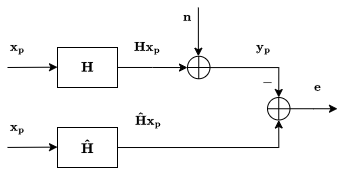
\includegraphics[width=0.65\linewidth]{../images/ls_block_diagram.png}
    \caption{Sơ đồ khối cho bộ ước lượng sai số bình phương tối thiểu}
\end{figure}

Mục tiêu của phương pháp ước lượng sai số bình phương tối thiểu là tìm một ma trận kênh truyền ước lượng \( \hat{\bm{H}} \) 
sao cho nó \textbf{giảm thiểu sai số bình phương} giữa tín hiệu thu thực tế \( \bm{y_p} \) và tín hiệu thu mong đợi \( \bm{\hat{H}} \bm{x_p} \). 
Sai số bình phương này có thể được định nghĩa qua hàm mất mát (loss function) như sau:

\[
\bm{J(\hat{H})} = \bm{e_1}^2 + \bm{e_2}^2 + ... + \bm{e_K}^2
\]
% 
\begin{equation}
    \bm{J(\hat{H})} = \| \bm{e} \|^2 = \| \bm{y_p} - \bm{\hat{H}}\bm{x_p} \|^2
\end{equation}

Trong đó:
\begin{itemize}
    \item \( \bm{y_p} - \bm{\hat{H}}\bm{x_p} \) là sai số giữa tín hiệu thu thực tế và tín hiệu thu mong đợi
    \item \( \|\cdot\|^2 \) là chuẩn bình phương Euclidean, đại diện cho tổng bình phương sai số giữa các phần tử của vector
\end{itemize}

Để tối thiểu hóa sai số bình phương, ta cần tìm ma trận kênh truyền \( \hat{\mathbf{H}} \) tối ưu. Điều này được thực hiện bằng cách giải phương trình tối ưu hóa sau:
%
\begin{equation}
    \bm{\hat{H}} 
    = \underset{\bm{\hat{H}}}{\arg \min} \; \bm{J(\hat{H})}
    = \underset{\bm{\hat{H}}}{\arg \min} \; \|\bm{y_p} - \bm{\hat{H}}\bm{x_p}\|^2
\end{equation}

\subsubsection{Tìm nghiệm tối ưu của ước lượng LS}

Trước hết, ta triển khai hàm mất mát \( \bm{J(\hat{H})} \): 
% 
\begin{align*}
    \bm{J(\hat{H})} 
    &= \| \bm{y_p} - \bm{\hat{H}}\bm{x_p} \|^2 \\
    &= (\bm{y_p} - \bm{\hat{H}}\bm{x_p})^H (\bm{y_p} - \bm{\hat{H}}\bm{x_p}) \\
    &= (\bm{y_p}^H - \bm{x_p}^H\bm{\hat{H}}^H) (\bm{y_p} - \bm{\hat{H}}\bm{x_p}) \\
    &= \bm{y_p}^H\bm{y_p} - \bm{y_p}^H\bm{\hat{H}}\bm{x_p} - \bm{x_p}^H\bm{\hat{H}}^H\bm{y_p} + \bm{x_p}^H\bm{\hat{H}}^H\bm{\hat{H}}\bm{x_p}
\end{align*}

Nghiệm tối ưu của phương pháp Least Squares có thể tìm được bằng cách cho gradient của hàm mất mát theo vector \( \bm{\hat{x}} \) bằng không:
% 
\begin{align*}
    \nabla_{\bm{\hat{H}}}\bm{J(\hat{H})}
    &= - \bm{y_p}\bm{x_p}^H + \bm{\hat{H}}\bm{x_p}\bm{x_p}^H = 0\\
    &\Leftrightarrow \bm{\hat{H}}\bm{x_p} = \bm{y_p}
\end{align*}

Vậy nghiệm tối ưu của kênh truyền ước lượng theo phương pháp LS là:
% 
\begin{equation}
    \bm{\hat{H}} = \bm{y_p}\bm{x_p}^H
\end{equation}

\textbf{Nhận xét}

Phương pháp Least Squares (LS) trong ước lượng kênh truyền vô tuyến có ưu điểm nổi bật là đơn giản và dễ triển khai. 
Phương pháp này không yêu cầu kiến thức sâu về thống kê hay xử lý tín hiệu, 
do đó rất phù hợp với các hệ thống có tài nguyên hạn chế. 
Hơn nữa, LS không cần thông tin về phân phối hay đặc tính của nhiễu, 
chỉ sử dụng tín hiệu huấn luyện và tín hiệu nhận được để ước lượng kênh. 
Trong điều kiện kênh truyền có tỷ lệ tín hiệu trên nhiễu cao, 
phương pháp này có thể mang lại kết quả khá chính xác.  

Tuy nhiên, LS tồn tại một số hạn chế quan trọng. 
Đầu tiên, nó rất nhạy cảm với nhiễu, đặc biệt trong các môi trường có SNR thấp. 
Do không xem xét tác động của nhiễu, kết quả ước lượng của LS thường bị suy giảm nghiêm trọng khi nhiễu mạnh xuất hiện. 
Thêm vào đó, LS không phải là một phương pháp tối ưu về mặt thống kê; 
các phương pháp khác như Minimum Mean Square Error (MMSE) thường cho kết quả tốt hơn nhờ tận dụng được thông tin thống kê của nhiễu. 
Ngoài ra, hiệu quả của LS còn phụ thuộc lớn vào tín hiệu huấn luyện. 
Nếu tín hiệu này không đủ mạnh hoặc bị lỗi, ước lượng kênh có thể không chính xác.

Phương pháp LS thường được sử dụng trong các ứng dụng không đòi hỏi cao về độ chính xác hoặc trong giai đoạn sơ bộ của ước lượng kênh. 
Nó cũng có thể được dùng làm bước khởi tạo cho các phương pháp tiên tiến hơn như MMSE hay các thuật toán dựa trên máy học. 
Để cải thiện hiệu suất của LS, ta có thể tối ưu độ dài và công suất của tín hiệu huấn luyện.

Phương pháp LS, mặc dù đơn giản, vẫn là một công cụ hữu ích trong nhiều tình huống. Tuy nhiên, để đạt hiệu suất cao hơn, nó thường được kết hợp với các kỹ thuật tiên tiến khác.

\subsubsection{Nội suy để ước lượng kênh tại các vị trí không phải pilot}

Phương pháp LS chỉ ước lượng được ma trận kênh \( \bm{H} \) tại các vị trí có ký tự pilot. 
Để tính toán giá trị kênh tại các vị trí không có ký tự pilot, các phương pháp \textbf{nội suy hai chiều} (2D interpolation) sẽ được sử dụng. 
Một số phương pháp nội suy phổ biến bao gồm:

\begin{itemize}
    \item Nội suy tuyến tính (Linear interpolation),
    \item Nội suy spline,
    \item Nội suy bậc cao (Higher-order interpolation).
\end{itemize}

Nội suy giúp tạo ra một ma trận kênh ước lượng đầy đủ tại tất cả các vị trí trong khung thời gian và tần số, dựa trên thông tin từ các vị trí pilot.